\documentclass[12pt]{article}
\usepackage{graphicx} % Required for inserting images
\usepackage{geometry}
\usepackage{amsmath}
\usepackage{hyperref}
\usepackage{amsmath}
\usepackage{enumitem}
\usepackage{amsfonts}
\usepackage{amssymb}
\usepackage{graphicx}
\usepackage{hyperref}
\usepackage{listings}
\usepackage{xcolor}
\usepackage{titling}
\usepackage{amsmath}
\usepackage{amssymb}
\usepackage{listings}
\usepackage{url}
\usepackage{tikz}
\usepackage{subcaption}
\usepackage{booktabs}
% Code listing style
\lstset{
    language=Python,
    basicstyle=\ttfamily\footnotesize,
    keywordstyle=\color{blue!60!black},
    stringstyle=\color{orange},
    commentstyle=\color{green!50!black},
    showstringspaces=false,
    breaklines=true,
    frame=single,
    numbers=left,
    numberstyle=\tiny\color{gray},
    tabsize=4,
    captionpos=b,
    backgroundcolor=\color{gray!10},
    rulecolor=\color{gray!30},
    frameround=tttt,
    escapeinside={(*}{*)}
}




\begin{document}

\title{Schur Numbers Week 14 Report}
\date{\today}
\begin{titlepage}
    \begin{center}
        \vspace*{1cm}

        \rule{\linewidth}{0.2mm} \\[0.4cm]
        {\Large \textbf{CSE 326 Analysis and Design of Algorithms }}\\[0.4cm]
        \textbf{Dr.Walid Gomaa}
 
        \rule{\linewidth}{0.2mm} \\[1.5cm]

        \begin{tabular}{c}
            \begin{tabular}{ll}
                \textbf{Name} & \textbf{ID} \\
                \hline
                Mohamed Abdelmonem Makram & 120220055 \\
                \hline
                Abdelrahman Ahmed Shaheen & 120220228 \\
                \hline
                Abdelrhman Mohamed Eldenary & 120220253 \\
                \hline
                Anas Ihab  Badr & 120220360 \\
                

            \end{tabular}
        \end{tabular}

        \vspace{1cm}

        

        \vspace{5cm}

        
\includegraphics[width=0.25\textwidth]{ejust.jpg}


        Computer Science Engineering Department\\
        Egypt-Japan University of Science and Technology\\

    \end{center}
\end{titlepage}


\tableofcontents
\newpage
\maketitle
Since this is the final report, we will be summarizing our journey through the Schur numbers problem. 

\section{The Beginning}
In the first couple of weeks, we focused on understanding the problem and the recent literature where we found the \textbf{Schur number five} paper published in 2017. This was the current state of the art for this problem where they used  massively parallel SAT solver, supported by new heuristics for decision-making and problem partitioning to find $S(5) = 160$ and prove it. However, they used too much computing power about 14 CPU years that was only achieved in 3 days using a Lonestar 5 that features 1252 Cray XC40 compute nodes, each equipped with two 12-core Intel Xeon processors, totaling 30,048 compute cores. Their problem is their solution is hardly scaclable to larger Schur numbers like $S(6)$ due to the exponential growth nature of the problem.

We tried exploring the problem on our own pace without using any supercomputers and with no external solving methods. We tried using multiprocessing, since it was one of the criteria said in the lecture, to have a parallelized solution. We used Python at first with some randomized algorithm, then C++ to try to brute force the problem for smaller numbers. Which worked for $S(3)$ and $S(4)$, but it took $S(4)$ about 5 minutes to solve. Our next step was to try and used CUDA, and the massive parallelization of the GPU to solve the problem.    \section{CUDA}
\subsection{Learning CUDA}
Since we had minimal experience with multiprocessing let alone CUDA, we had to learn at least the basics of how CUDA can be used to solve problems. We understood various concepts like how the data is copied from and to the GPU, how the threads are organized in blocks and grids, and how to use shared memory. Our first CUDA program at week 6 was just trying to check the validity of a coloring where each thread would check a color individually. This was not a very big difference, but it was a start. 
\subsection{Novel encoding approach}
After some weeks with no idea what we were doing, a brilliant idea came to us. Traversing the problem as a tree in a DFS manner. We introduced a novel bit mask encoding approach to represent the coloring as 2 64-bit integers for each color such that each bit is turned on in only one color which represents the color of the index of that bit. For example a coloring like this: 

\begin{align*}
\centering
C_0 &= \texttt{0000001001001001}_2 \\
C_1 &= \texttt{0000000100010010}_2 \\
C_2 &= \texttt{0000000010100100}_2 \\
\end{align*}
would mean that the number 1, 4, 7, 10 are colored using $C_0$, the number 2, 5, 9 are colored using $C_1$, and the number 3, 6, 8 are colored using $C_2$ (We used 2 64-bit integers to represent number from 1 to 128). This allowed for less memory usage, faster access, and faster validation of the coloring. Then for traversing the problem, we would initiate a coloring of length 4. Then our algorithm would be as follows:
\begin{enumerate}
    \item Iterate through all the current coloring in \texttt{current\_states} in a parallelized manner. (starting with one coloring)
    \item Check if the next number can be colored with any color in the previous coloring.
    \item If yes, store the coloring with the new number in \texttt{next\_states} buffer and continue.
\end{enumerate}  
This way we check all the possible colorings while utilizing the GPU threads to check for valid next state colorings. A diagram of the tree is shown in \texttt{tex/images/recursionTree.png} (it was too large to fit in the pdf).

The code preformed very well and we could obtain $S(4)$ in 30 ms compared to 5 minutes in Python. 
\begin{figure}[h]
    \centering
    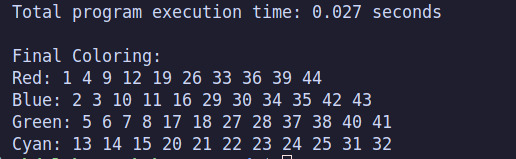
\includegraphics[width=0.8\textwidth]{images/finalCUDAwithTime.jpeg}
    \caption{CUDA code output}
    \label{fig:CUDA_time}
\end{figure}

\subsection{Scaling the algorithm}
\subsection{Initial attempt}
We then tried to scale the algorithm to $S(5)$, by using 3 64-bit integers to represent number from 1 to 192 (as $S(5)$ is 160). We only reached a coloring of length \textbf{81} before we ran out of memory to represent all the states (Over 37 million states). But this was not bad at all. Compared to what took the people from the Schur number five paper, this was quite impressive. 

\subsection{Randomized Monte Carlo}
Since we didn't need all the states from the beginning, we decided to try a randomized approach where we would use Monte Carlo rollouts on the CPU to generate diverse partial colorings up to a fixed depth, and then offloads successful rollouts to the GPU, where we do our breadth-first search normally with fewer states. After that randomized approach, we saw a huge improvement where we could reach a coloring of length \textbf{113} before we ran out of memory again. This was a huge improvement, and we were very happy with the results. 
\begin{figure}
    \centering
    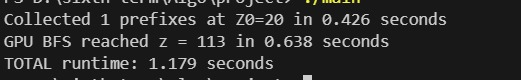
\includegraphics[width=0.8\textwidth]{images/montecarlo.jpg}
    \caption{Monte Carlo approach}
    \label{fig:monteCarlo}
\end{figure}


\section{Reinforcement Learning and Transformers}
Although our parallelized approach was promising, and we could reach a coloring of length 113 with using only our laptops, we had the passion to try and use something that didn't exist in 2017. We wanted to try and use reinforcement learning to solve the problem. We believed that this may be a very good approach, since it was something unexplored in the Schur numbers problem, and that maybe we are on the verge of a breakthrough (we were not).  

\subsection{Reinforcement Learning}
What first came to mind when we draw our \texttt{recursionTree} diagram is that it was too similar to what Google DeepMind did with AlphaGo (Figure \ref{fig:alphaGO}). They used a Monte Carlo tree search to traverse the game tree and then used a neural network to evaluate the states. We though the same logic could be applied to our problem. We could use a Monte Carlo tree search to traverse our states, evaluate the states according to how deep they managed to get the tree to, and design our reward function to be proportional to the depth of the tree. 
\begin{figure}[h]
    \centering
    \includegraphics[width=0.8\textwidth]{images/AlphaGo.png}
    \caption{AlphaGo model}
    \label{fig:alphaGO}
\end{figure}

Again, we had minimal experience with reinforcement learning, but we tried implementing the mentioned algorithm in a very short time. The results were not that great achieving only colorings of length 28. But to think that it reached there from scratch was no data is still quite impressive. 

\subsection{Transformers}
With a novel idea this time, we thought of treating the problem as a sequence of numbers and colors where the transformers should be able to learn the patterns of the colorings without finding a monochromatic solution to the equation $x + y = z$. This time we generated our own dataset of colorings using the CUDA code we wrote before.
We generated 1000 coloring for each depth from 1 to 70 (the maximum our initial CUDA approach could reach) then we initially used an encoder only transformers to try to understand the nature of the sequence and come up with the next color. The transformer processes variable-length sequences by embedding the numbers and their corresponding colors separately, then concatenating them into unified token representations. A learned positional encoding is added to help the model understand sequence order. The core of the architecture is a lightweight multi-head, multi-layer Transformer encoder, and the output corresponding to the last token is passed through a linear layer and softmax to produce a probability distribution over the five possible colors. The model is trained using a standard cross-entropy loss on valid color predictions.
Each training example is a prefix of a sequence, and the target is the color of the next
number. After training the transformer locally the results were somehow decent. In figure \ref{fig:transformer} it shows the results of taking the average output length the transformer could reach for 500 trials for each input length from 6 to 70.
\begin{figure}[h]
    \centering
    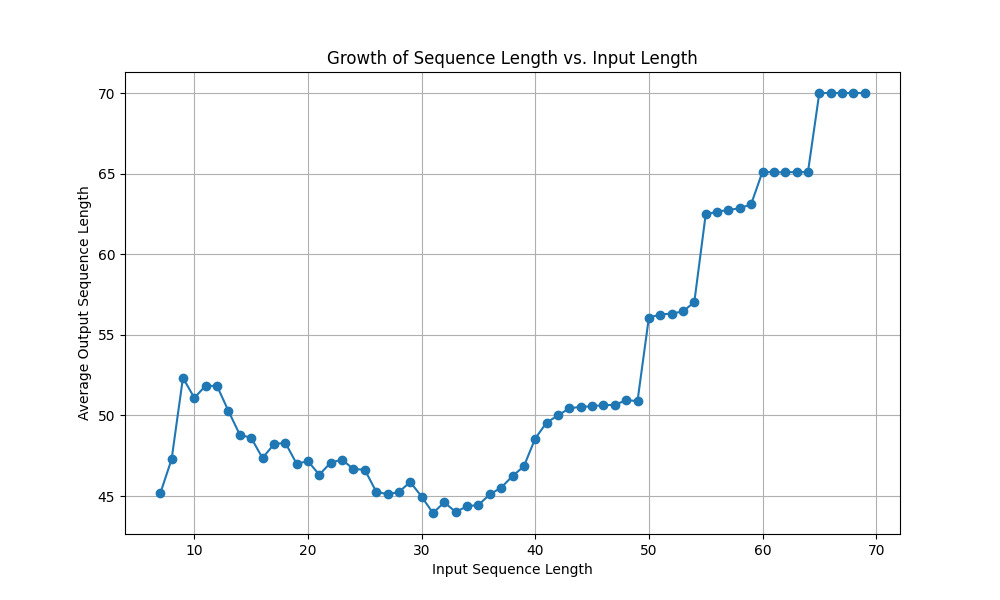
\includegraphics[width=0.8\textwidth]{images/TransformerOnly.png}
    \caption{Transformer model results}
    \label{fig:transformer}
\end{figure} 
In this final week we tried to fine tune the transformer that has some good initial predictions using Reinforcement learning to try to improve its results. We ussed PPO


\end{document}